\section{Image Interpolation}
Measuring the strength of the image interpolation algorithm objectively is difficult. This also makes the design and improvement of filters a difficult process, as a filter scheme which seems to work well for one image will not work well for another. The field of computer vision is one that attempts to deal with these problems, but a rigorous implementation of algorithms within this field was not the main focus of our implementation. Our objective was to create a filtering system which gave a reasonable and recognisable output for any given input and as such a very general and robust edge capturing algorithm was designed. Arguably the best way to measure the performance of the algorithm is to compare its effectiveness objectively against a range of different input images. A comparison of a selection of inputs and outputs can be seen in Figure \ref{fig:imageInterpolation}.

\begin{figure}[htbp]  
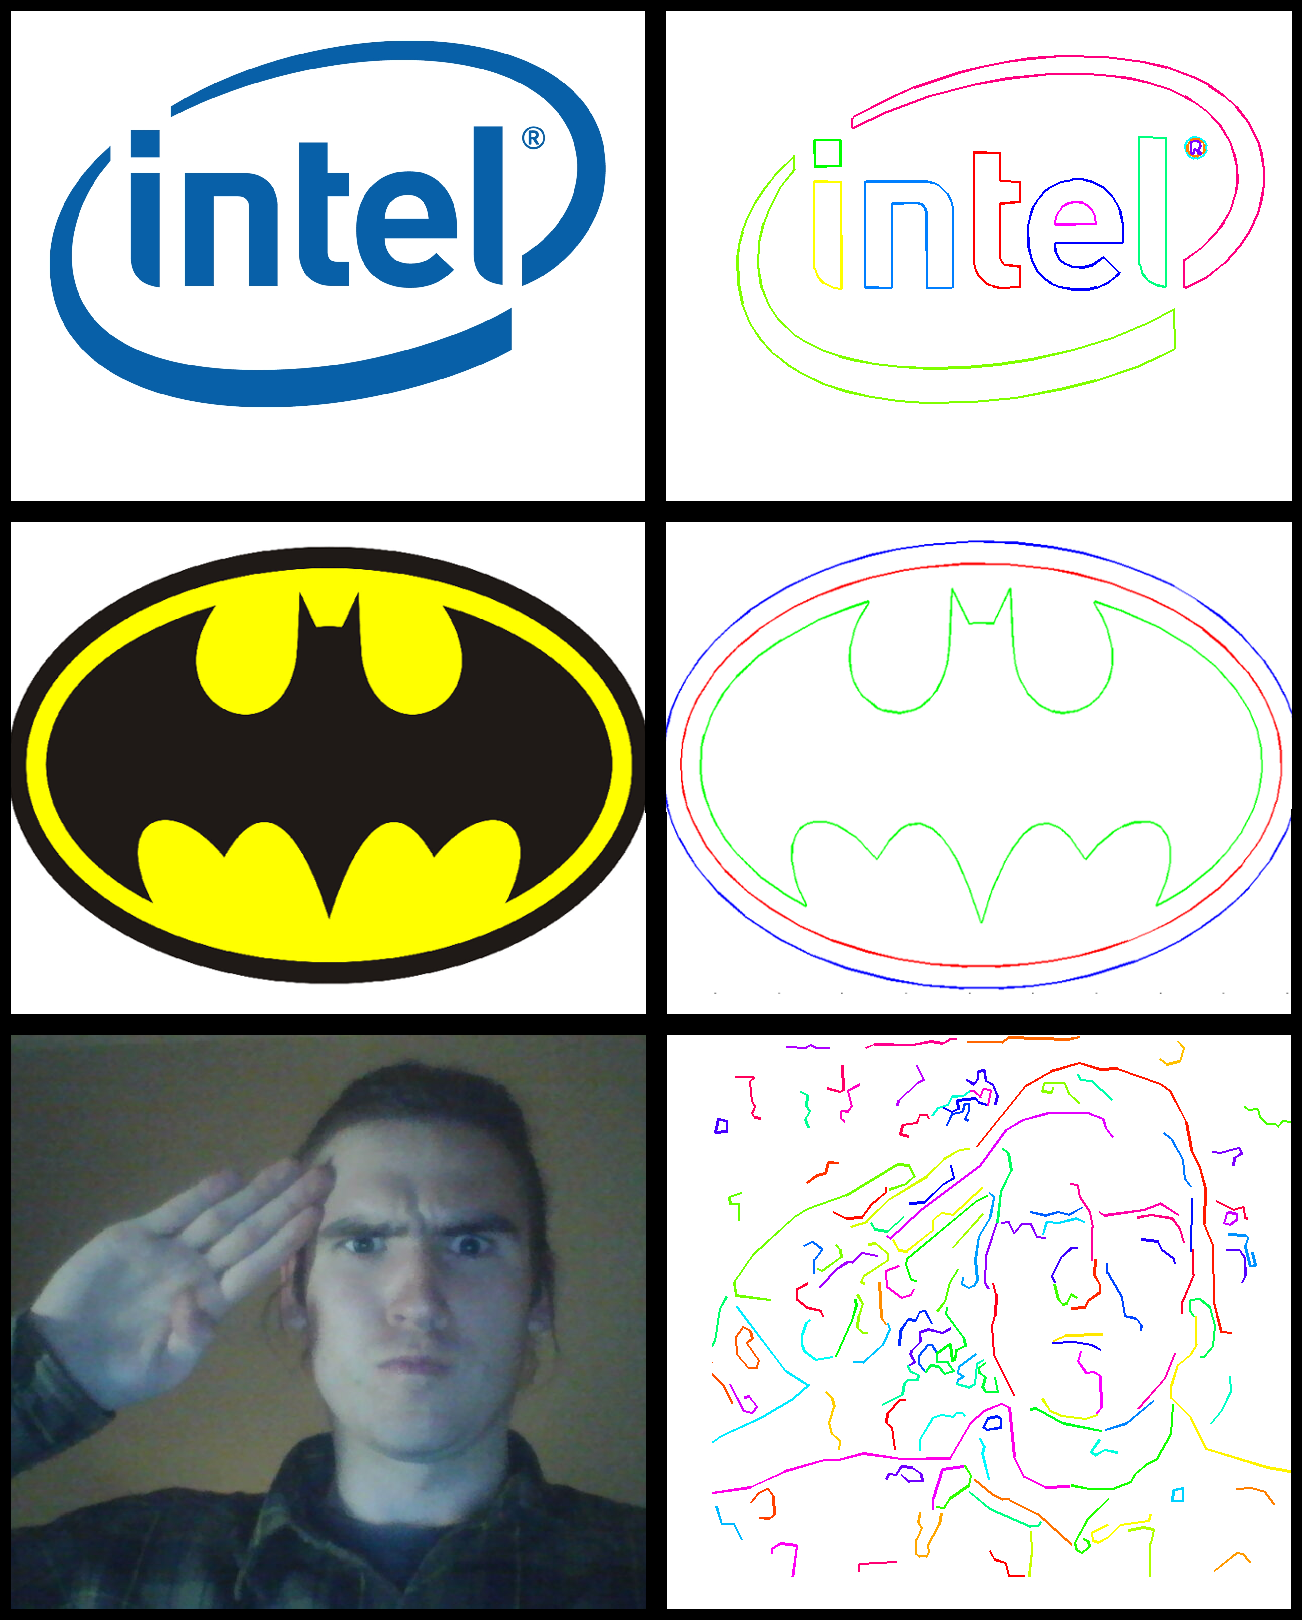
\includegraphics[width=\textwidth]{figures/performance/imageInterpolation.png}
\caption[Examples of image interpolation performance]{Examples of image interpolation performance. LEFT: Image before processing. RIGHT: Plot of the curves extracted from the image.
\label{fig:imageInterpolation}}
\end{figure}

When there are obvious lines to be found, the image filter does an excellent job of finding those lines and composing the image out of them. However, in more complex images such as the colour photo of a face, noise abounds and the many edges are detected in the image. This problem is one that remains generally unsolved in image filtering and arguably there is no correct mapping from an image to a set of contours. Within respect to the intended purpose of the algorithm, simple images or vector drawings are easily imported and are represented very well by the filter. Complex images will have mixed results, but the general gist of the image will be conveyed.
